\chapter{Software Design} \label{ch:SwDesign}

\section{Version}
\begin{table}[h]
	\centering
	\begin{tabularx}{\textwidth - 2cm}{|l|l|l|X|}
	\hline
	Dato	& Version	& Initialer & Ændring	\\ \hline
	29. marts & 1 & KS & Første udkast. \\ \hline 
	\end{tabularx}
\end{table}

\section{Indledning}
%TODO Skriv en indledning?

\section{Udvidet Applikationsmodel: Sekvensdiagrammer}

\subsection{Usecase 1: Start}

\begin{figure}[!h]
\centering 
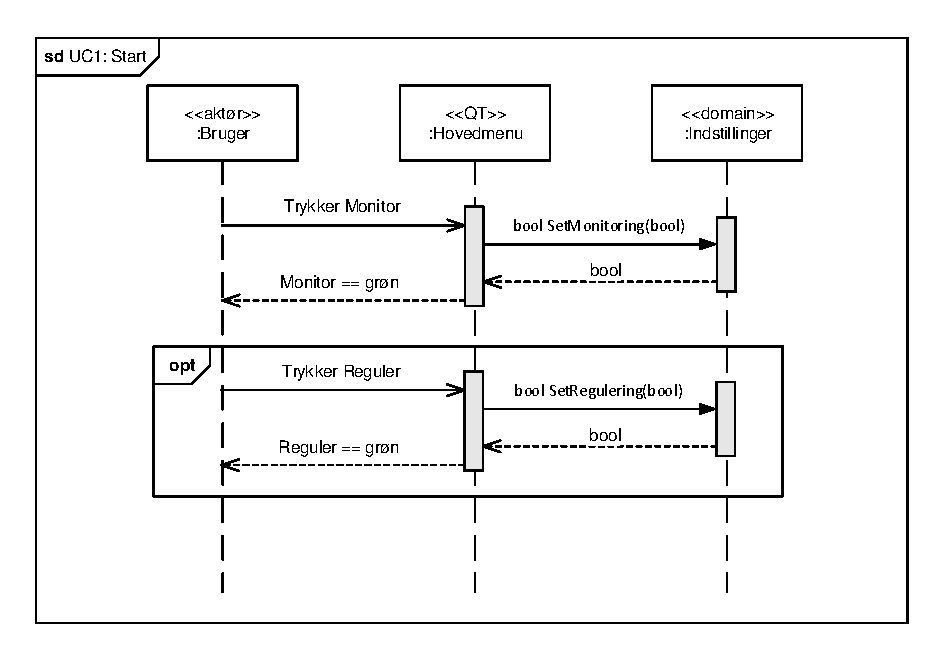
\includegraphics[width={\textwidth}, trim=0 0 0 0, clip=true] {../fig/SD_autoGreen_UC_1_Start.pdf}
\caption{Application model for UC1: Start}
\label{fig:SD_UC1}
\end{figure}

Sekvensdiagrammet for start er funktionaliten der skal forgå når der startes for monitorering, og også funktionaliteten for regulator hvis den også tændes.

\clearpage

\subsection{Usecase 2: Stop}

\begin{figure}[!h]
\centering 
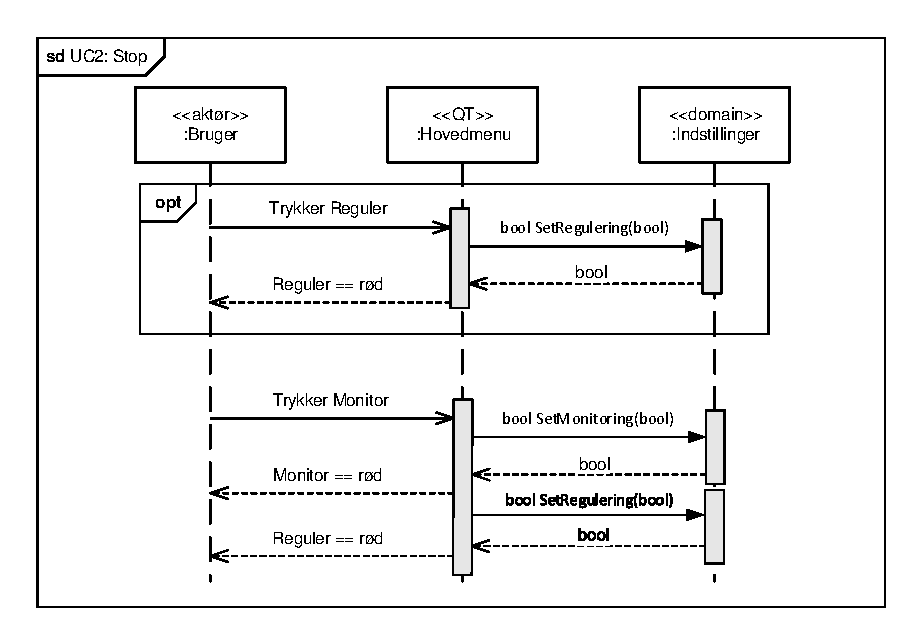
\includegraphics[width={\textwidth}, trim=0 0 0 0, clip=true] {../fig/SD_autoGreen_UC_2_Stop.pdf}
\caption{Application model for UC2: Stop}
\label{fig:SD_UC2}
\end{figure}

Sekvensdiagrammet for stop, når der ønskes at stoppe for monitorering og/eller regulering. Tryk på monitorering på begge er tændt, resultere i at både regulator og monitor slukkes.

\clearpage

\subsection{Usecase 4: Administrer Drivhus}

\begin{figure}[!h]
\centering 
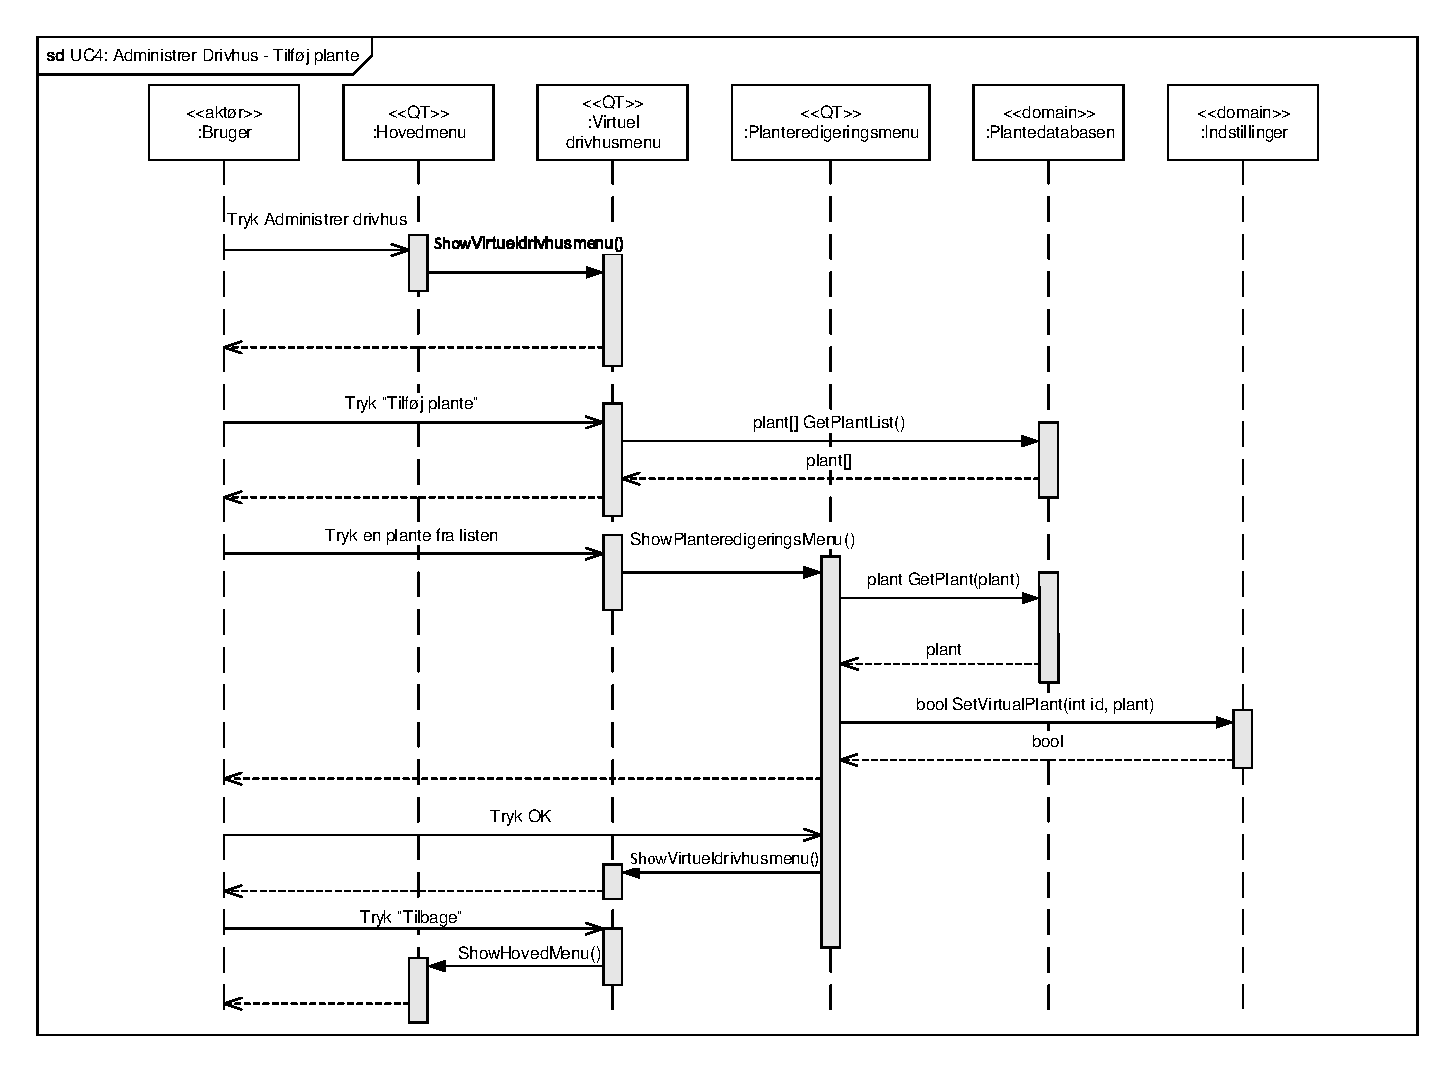
\includegraphics[width={\textwidth}, trim=0 0 0 0, clip=true] {../fig/SD_autoGreen_UC_4_Administrerdrivhus.pdf}
\caption{Application model for UC4: Administrer Drivhus - Tilføj Plante}
\label{fig:SD_UC4}
\end{figure}

Adminstre drivhus sekvensdiagrammet giver overblik over hvad der fortages når der ønskes at tilføje en plante igennem det virtuelle drivhus.

\clearpage

\begin{figure}[!h]
\centering 
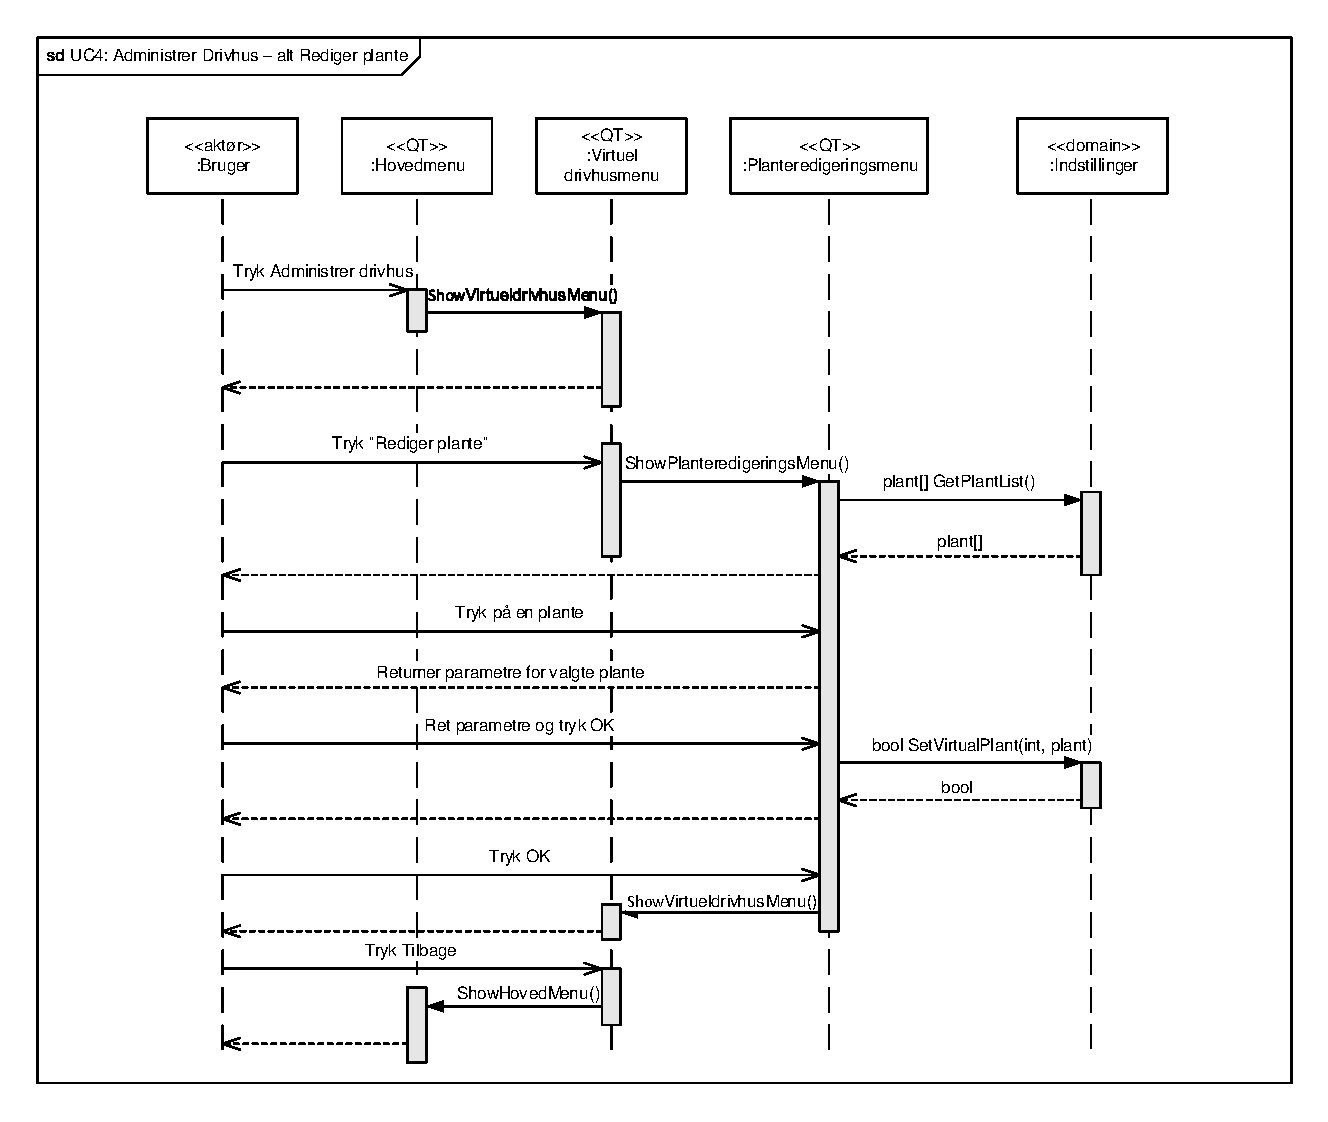
\includegraphics[width={\textwidth}, trim=0 0 0 0, clip=true] {../fig/SD_autoGreen_UC_4_Administrerdrivhus_alt_redigerplante.pdf}
\caption{Application model for UC4: Administrer Drivhus - [alt] Rediger Plante}
\label{fig:SD_UC4_alt1}
\end{figure}

Sekvensdiagrammet giver overblik over hvad der fortages i softwaren, når det ønskes at redigere en af de allerede tilstedeværende planter i det virtuelle drivhus.

\clearpage

\begin{figure}[!h]
\centering 
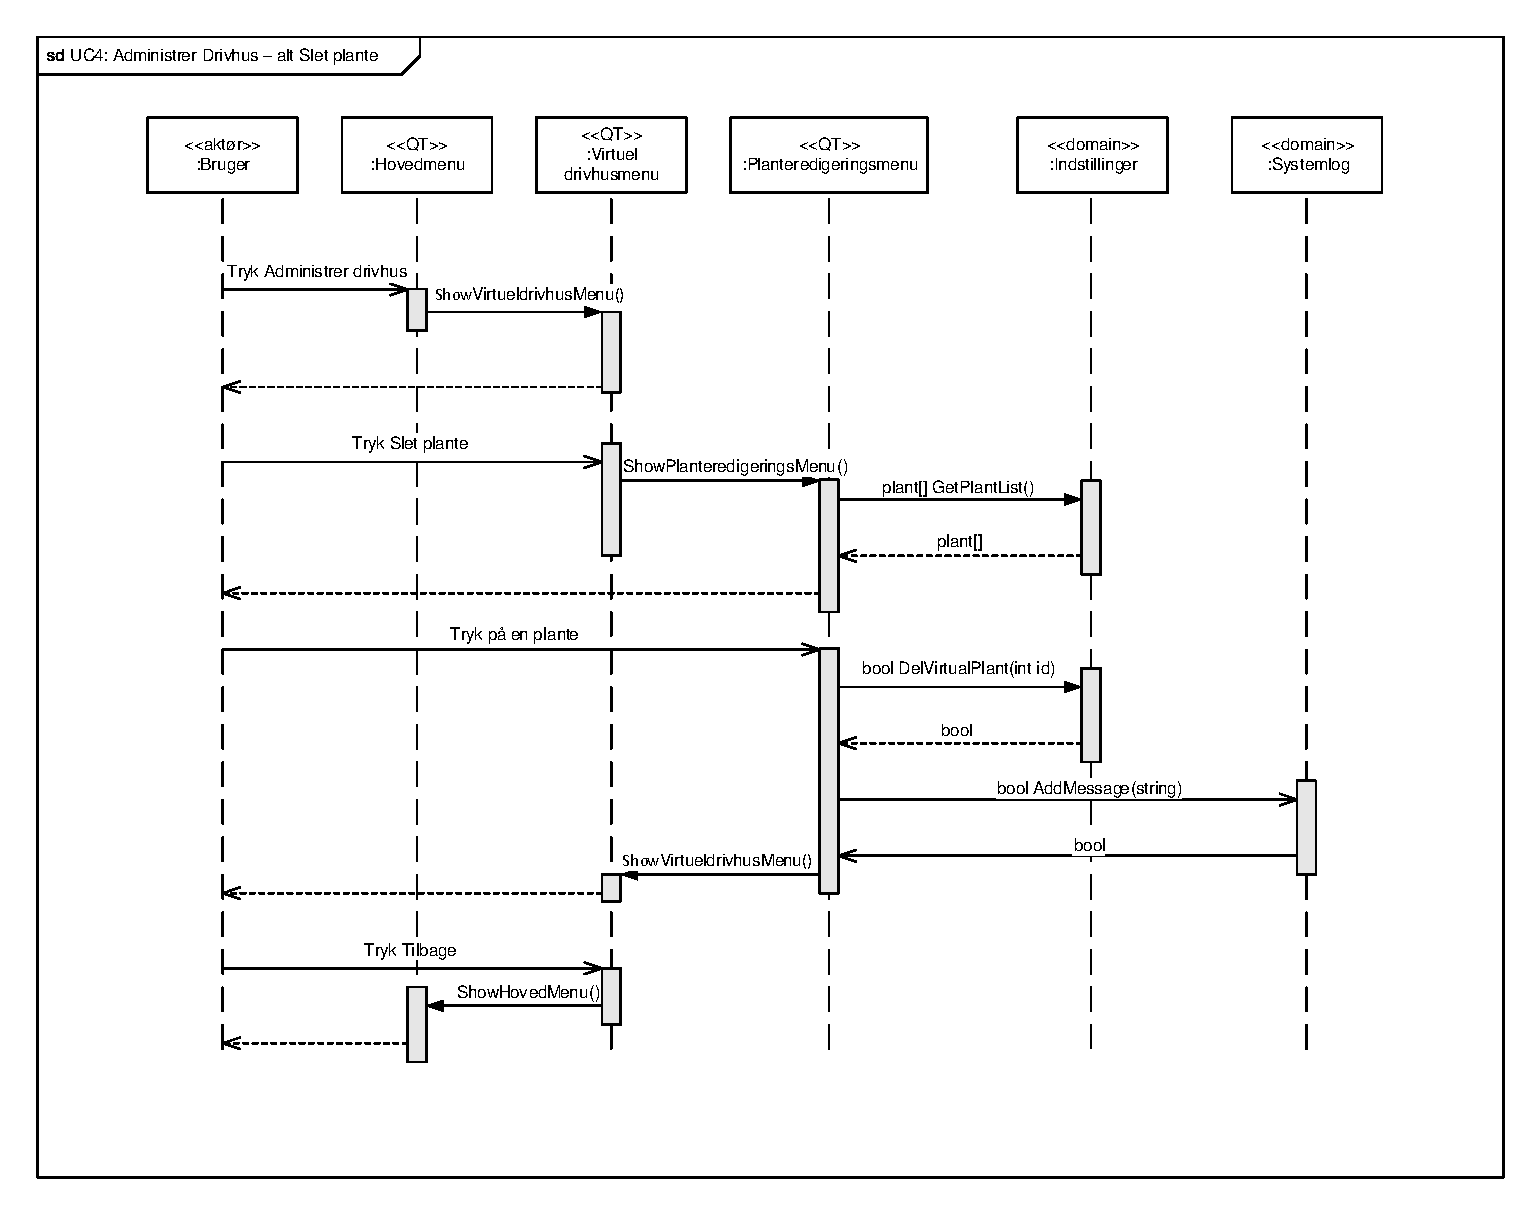
\includegraphics[width={\textwidth}, trim=0 0 0 0, clip=true] {../fig/SD_autoGreen_UC_4_Administrerdrivhus_alt_sletplante.pdf}
\caption{Application model for UC4: Administrer Drivhus - [alt] Slet Plante}
\label{fig:SD_UC4_alt2}
\end{figure}

Sekvensdiagrammet giver overblik over hvad der fortages i softwaren, når det ønskes at fjerne en tilstedeværende plante fra det virtuelle drivhus.

\clearpage

\subsection{Usecase 5: Vis Historik}

\begin{figure}[!h]
\centering 
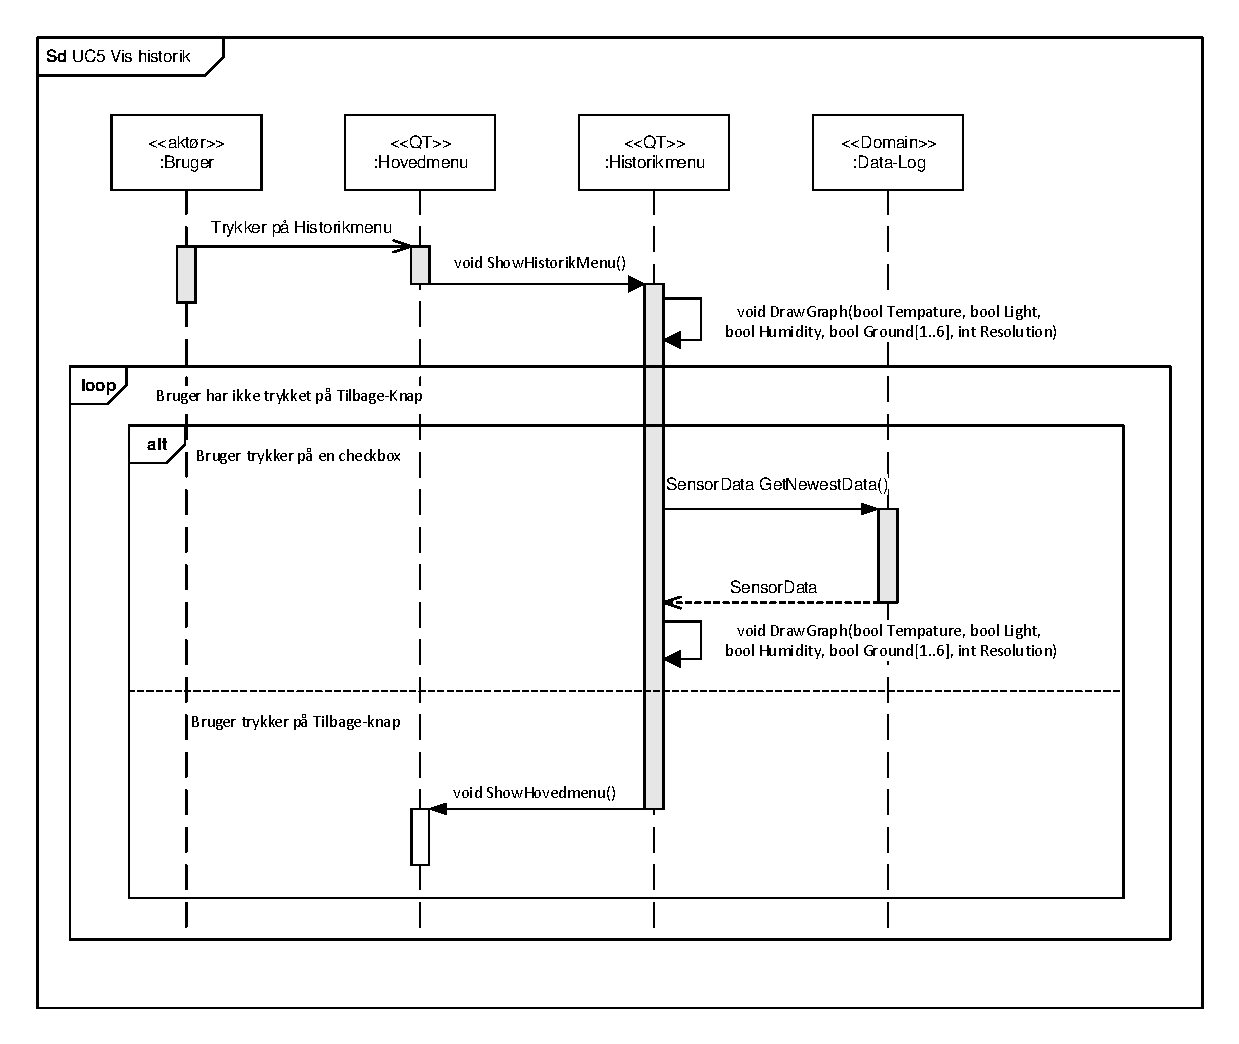
\includegraphics[width={\textwidth}, trim=0 0 0 0, clip=true] {../fig/SD_autogreen_UC_5_Vis_historik.pdf}
\caption{Application model for UC5: Vis Historik}
\label{fig:SD_UC5}
\end{figure}

Sekvensdiagrammet giver overblik over hvordan historiken fungerer, når brugeren trykker ind på 'se historik' igennem hovedmenuen.

\clearpage

\subsection{Usecase 6: Adminstrer Plantedatabase}

\begin{figure}[!h]
\centering 
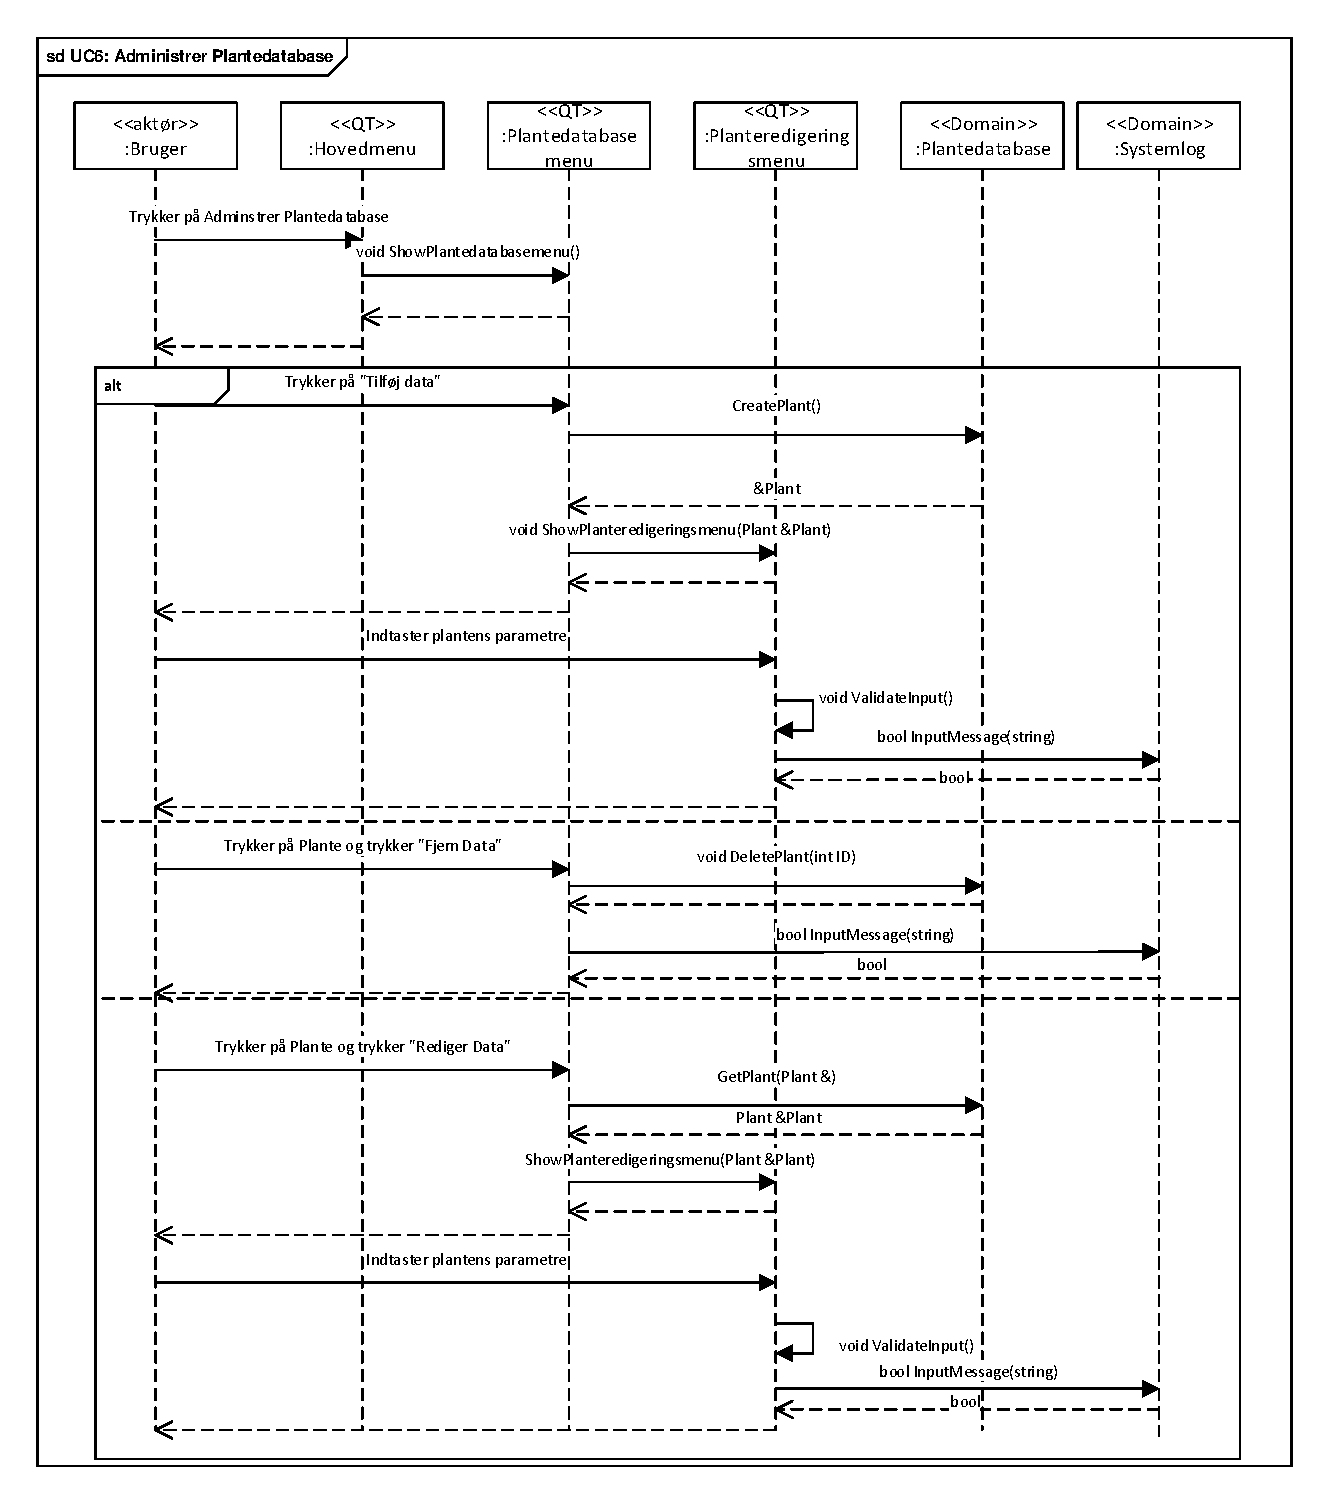
\includegraphics[width={\textwidth}, trim=0 0 0 0, clip=true] {../fig/SD_autogreen_UC_6_Adminstrer_Plantedatabase.pdf}
\caption{Application model for UC6: Administerer Plantedatabase}
\label{fig:SD_UC6}
\end{figure}

Sekvensdiagrammet giver overblik over de forskellige muligheder brugeren skal have inde fra plantedatabasen, hvorvidt en plante skal tilføjes, redigeres eller slettes.

\clearpage

\subsection{Usecase 7: Konfigurer System}

Når brugeren går ind på indstillingsmenuen bliver brugeren mødt med 4 undermenu som kan tilgåes, hertil er sekvensdiagrammerne for disse menuer.

\begin{figure}[!h]
\centering 
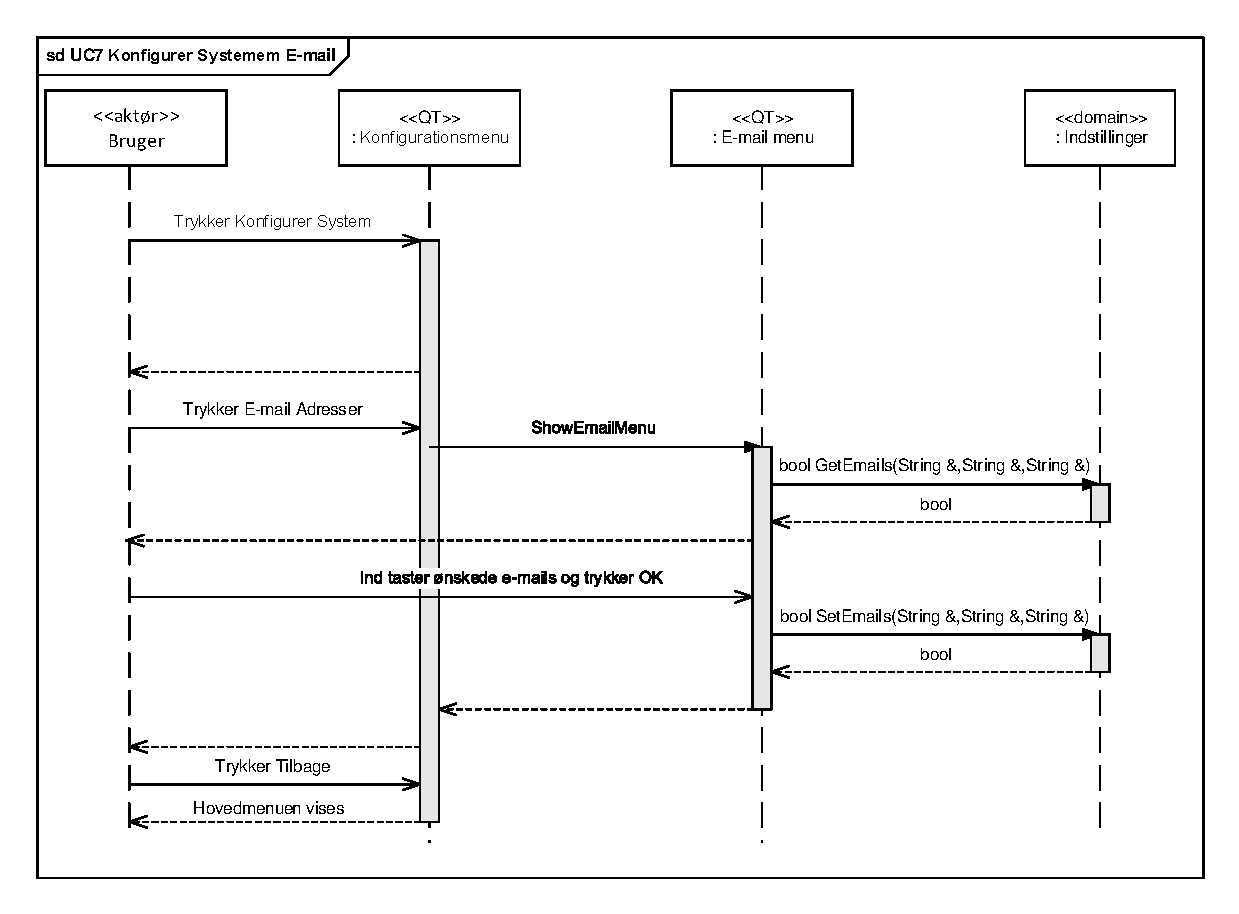
\includegraphics[width={\textwidth}, trim=0 0 0 0, clip=true] {../fig/SD_autoGreen_UC_7_E_mail.pdf}
\caption{Application model for UC7: Konfigurer System - E-mail}
\label{fig:SD_UC7}
\end{figure}

sekvensdiagrammet giver overblik over, hvordan brugeren kan skifte E-mails igennem E-mail menuen.

\clearpage

\begin{figure}[!h]
\centering 
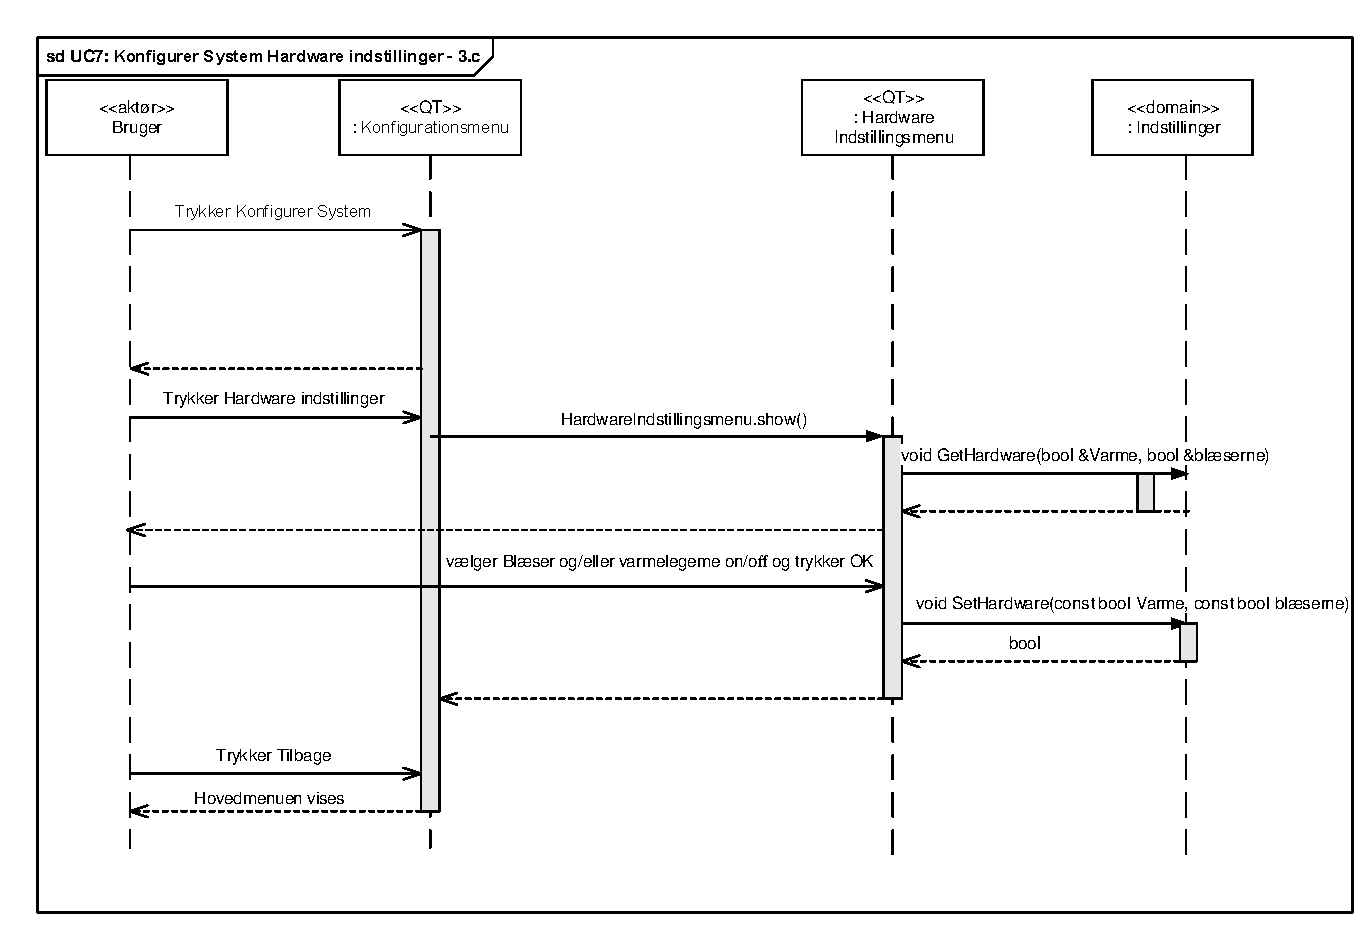
\includegraphics[width={\textwidth}, trim=0 0 0 0, clip=true] {../fig/SD_autoGreen_UC_7_Hardware_indstillinger.pdf}
\caption{Application model for UC7: Konfigurer System - Hardware Indstillinger}
\label{fig:SD_UC7_alt1}
\end{figure}

sekvensdiagrammet giver overblik over, hvordan brugeren kan skifte hardware indstillinger. Brugeren kan her vælge om blæsere og varmelegeme skal anvendes under regulering.

\clearpage

\begin{figure}[!h]
\centering 
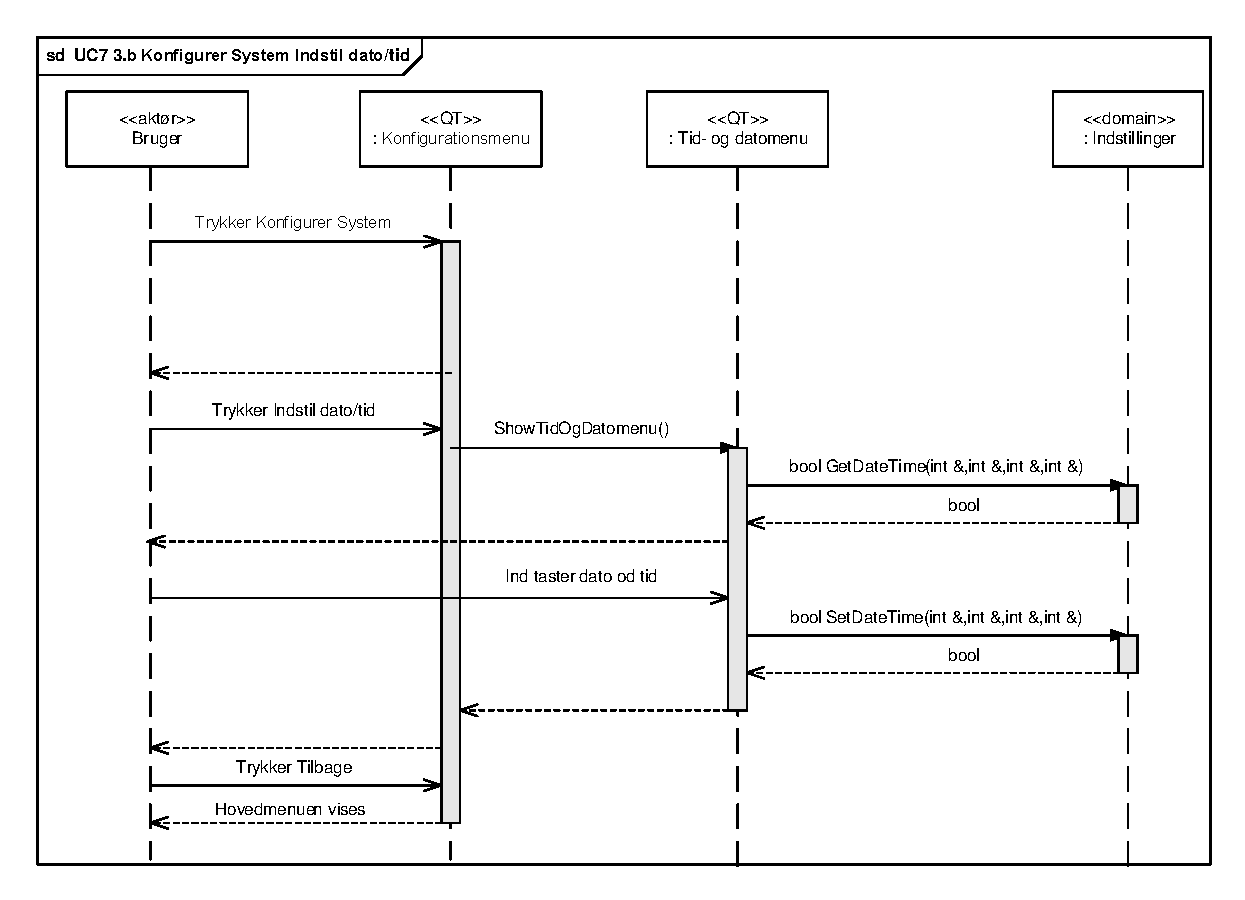
\includegraphics[width={\textwidth}, trim=0 0 0 0, clip=true] {../fig/SD_autoGreen_UC_7_Indstil_dato_tid.pdf}
\caption{Application model for UC7: Konfigurer System - Dato/Tid}
\label{fig:SD_UC7_alt2}
\end{figure}

Sekvensdiagrammet giver overblik over, hvordan brugeren kan indstille tiden på systemet.

\clearpage

\begin{figure}[!h]
\centering 
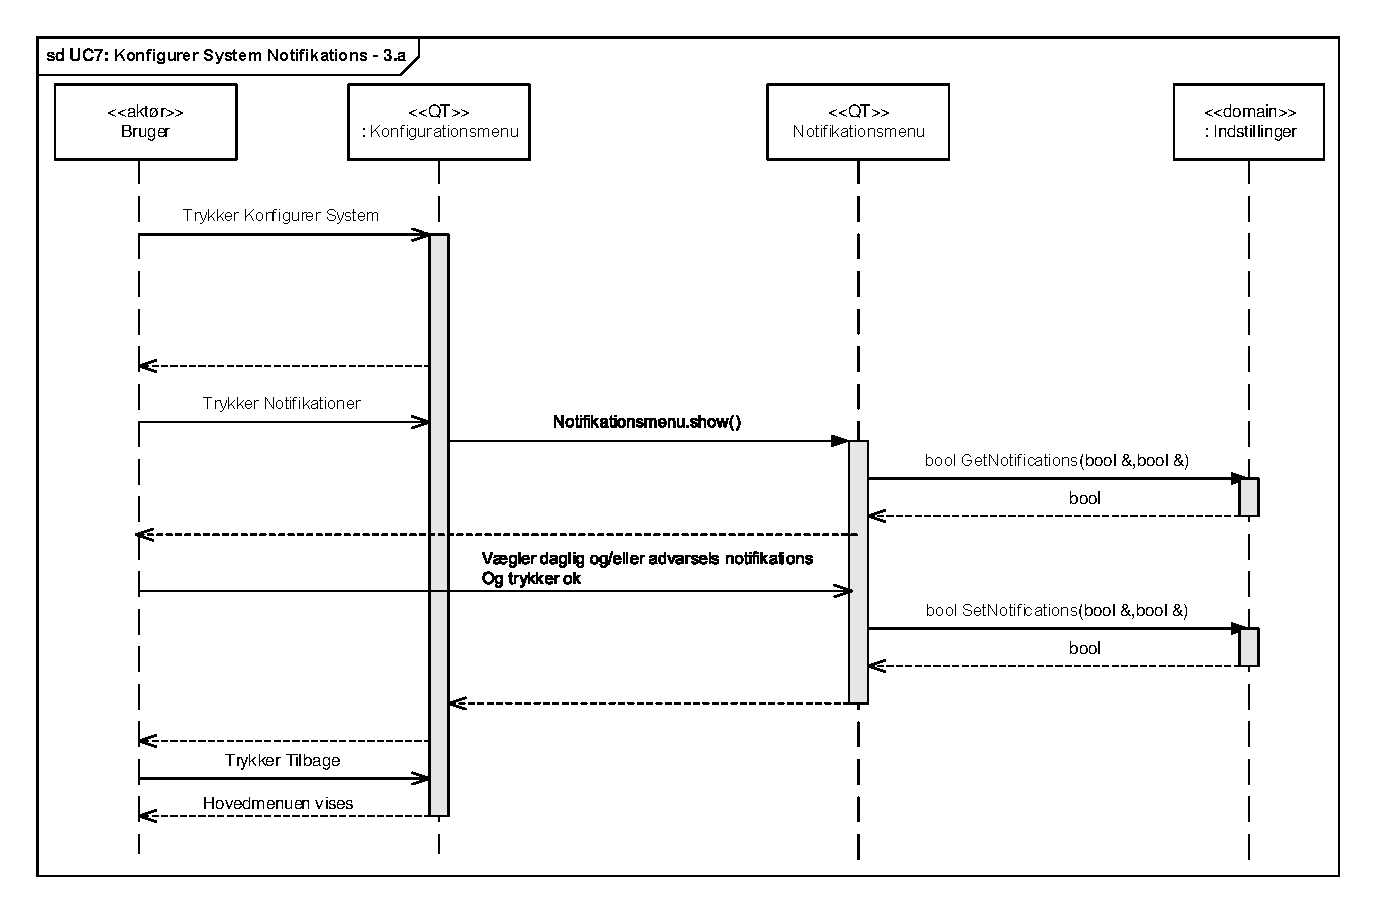
\includegraphics[width={\textwidth}, trim=0 0 0 0, clip=true] {../fig/SD_autoGreen_UC_7_Notifikationer.pdf}
\caption{Application model for UC7: Konfigurer System - Notifikation}
\label{fig:SD_UC7_alt3}
\end{figure}

Sekvensdiagrammet giver overblik over, hvordan brugeren kan aktivere og deaktivere brugen af daglige og vigtige notifikations emails fra system.

\clearpage

\subsection{Usecase 8: Se Systemlog}

\begin{figure}[!h]
\centering 
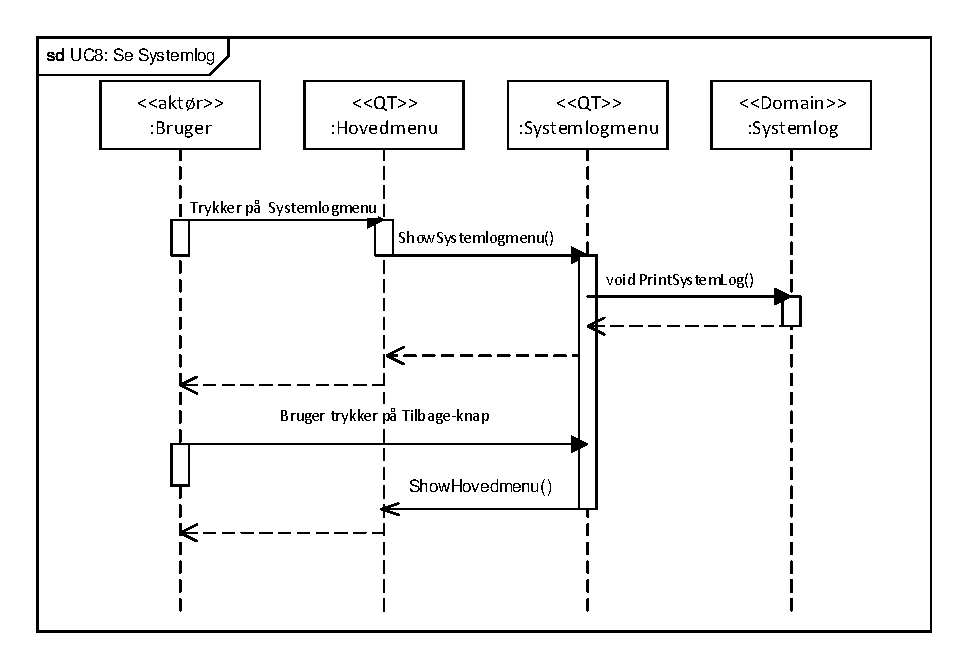
\includegraphics[width={\textwidth}, trim=0 0 0 0, clip=true] {../fig/SD_autogreen_UC_8_Se_Systemlog.pdf}
\caption{Application model for UC8: Se Systemlog}
\label{fig:SD_UC8}
\end{figure}

Sekvensdiagrammet giver overblik over hvordan brugeren kan tilgå systemloggen igennem dens egen menu. Når brugeren har tilgået menuen, udskrives de seneste systemhændelser på skærmen.

\clearpage

\subsection{Usecase 9: Rapportering}

\begin{figure}[!h]
\centering 
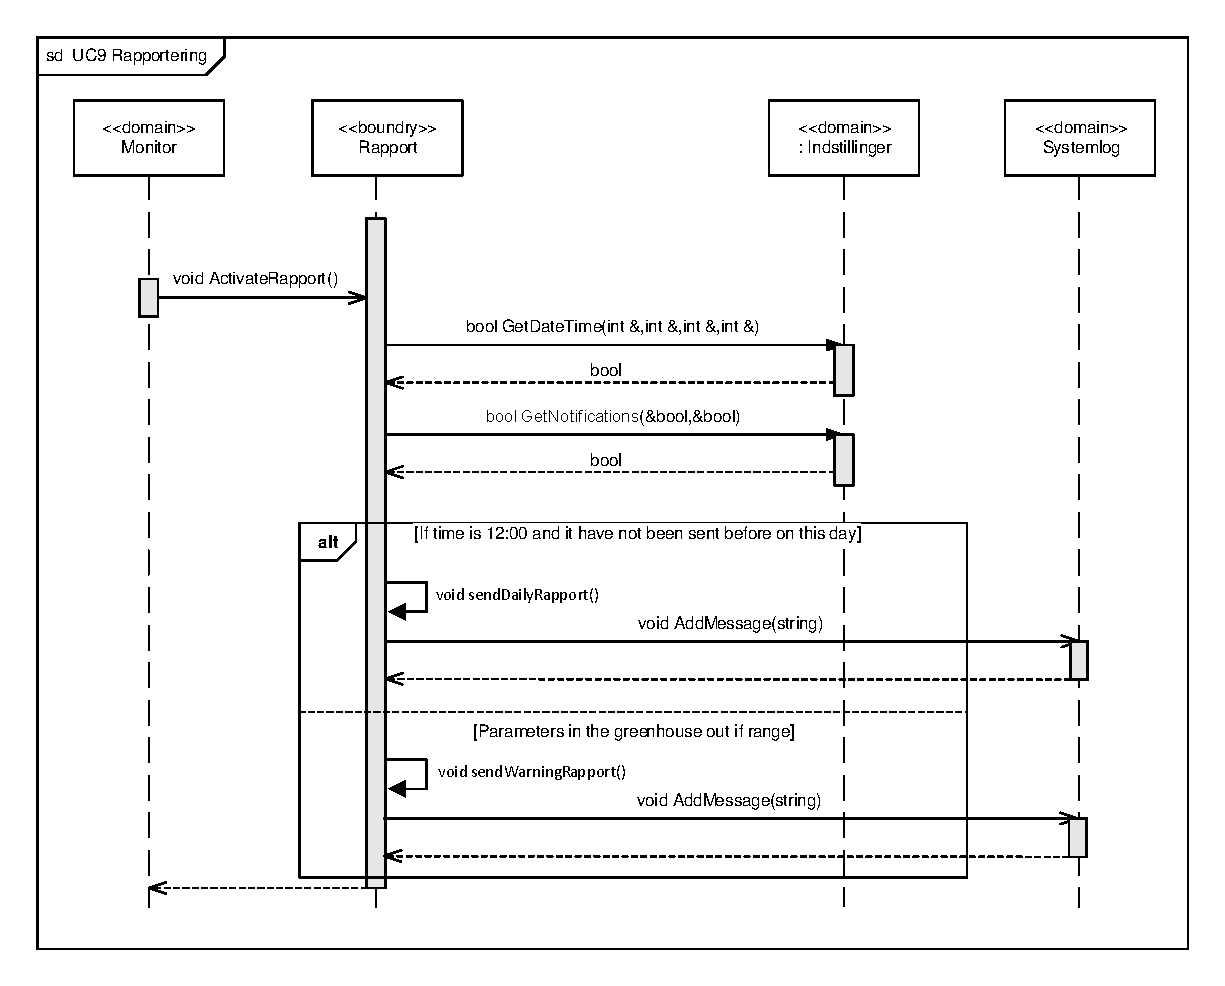
\includegraphics[width={\textwidth}, trim=0 0 0 0, clip=true] {../fig/SD_autoGreen_UC_9_Rapportering.pdf}
\caption{Application model for UC9: Rapportering}
\label{fig:SD_UC9}
\end{figure}

Sekvensdiagrammet giver overblik over, hvordan systemet kan bruger rapportering til at udsende emails til bruger, om den skal sende daglige, kun vigtige eller ingen email hentes ind fra indstillinger.

\clearpage

\subsection{Usecase 10: Monitorering}

\begin{figure}[!h]
\centering 
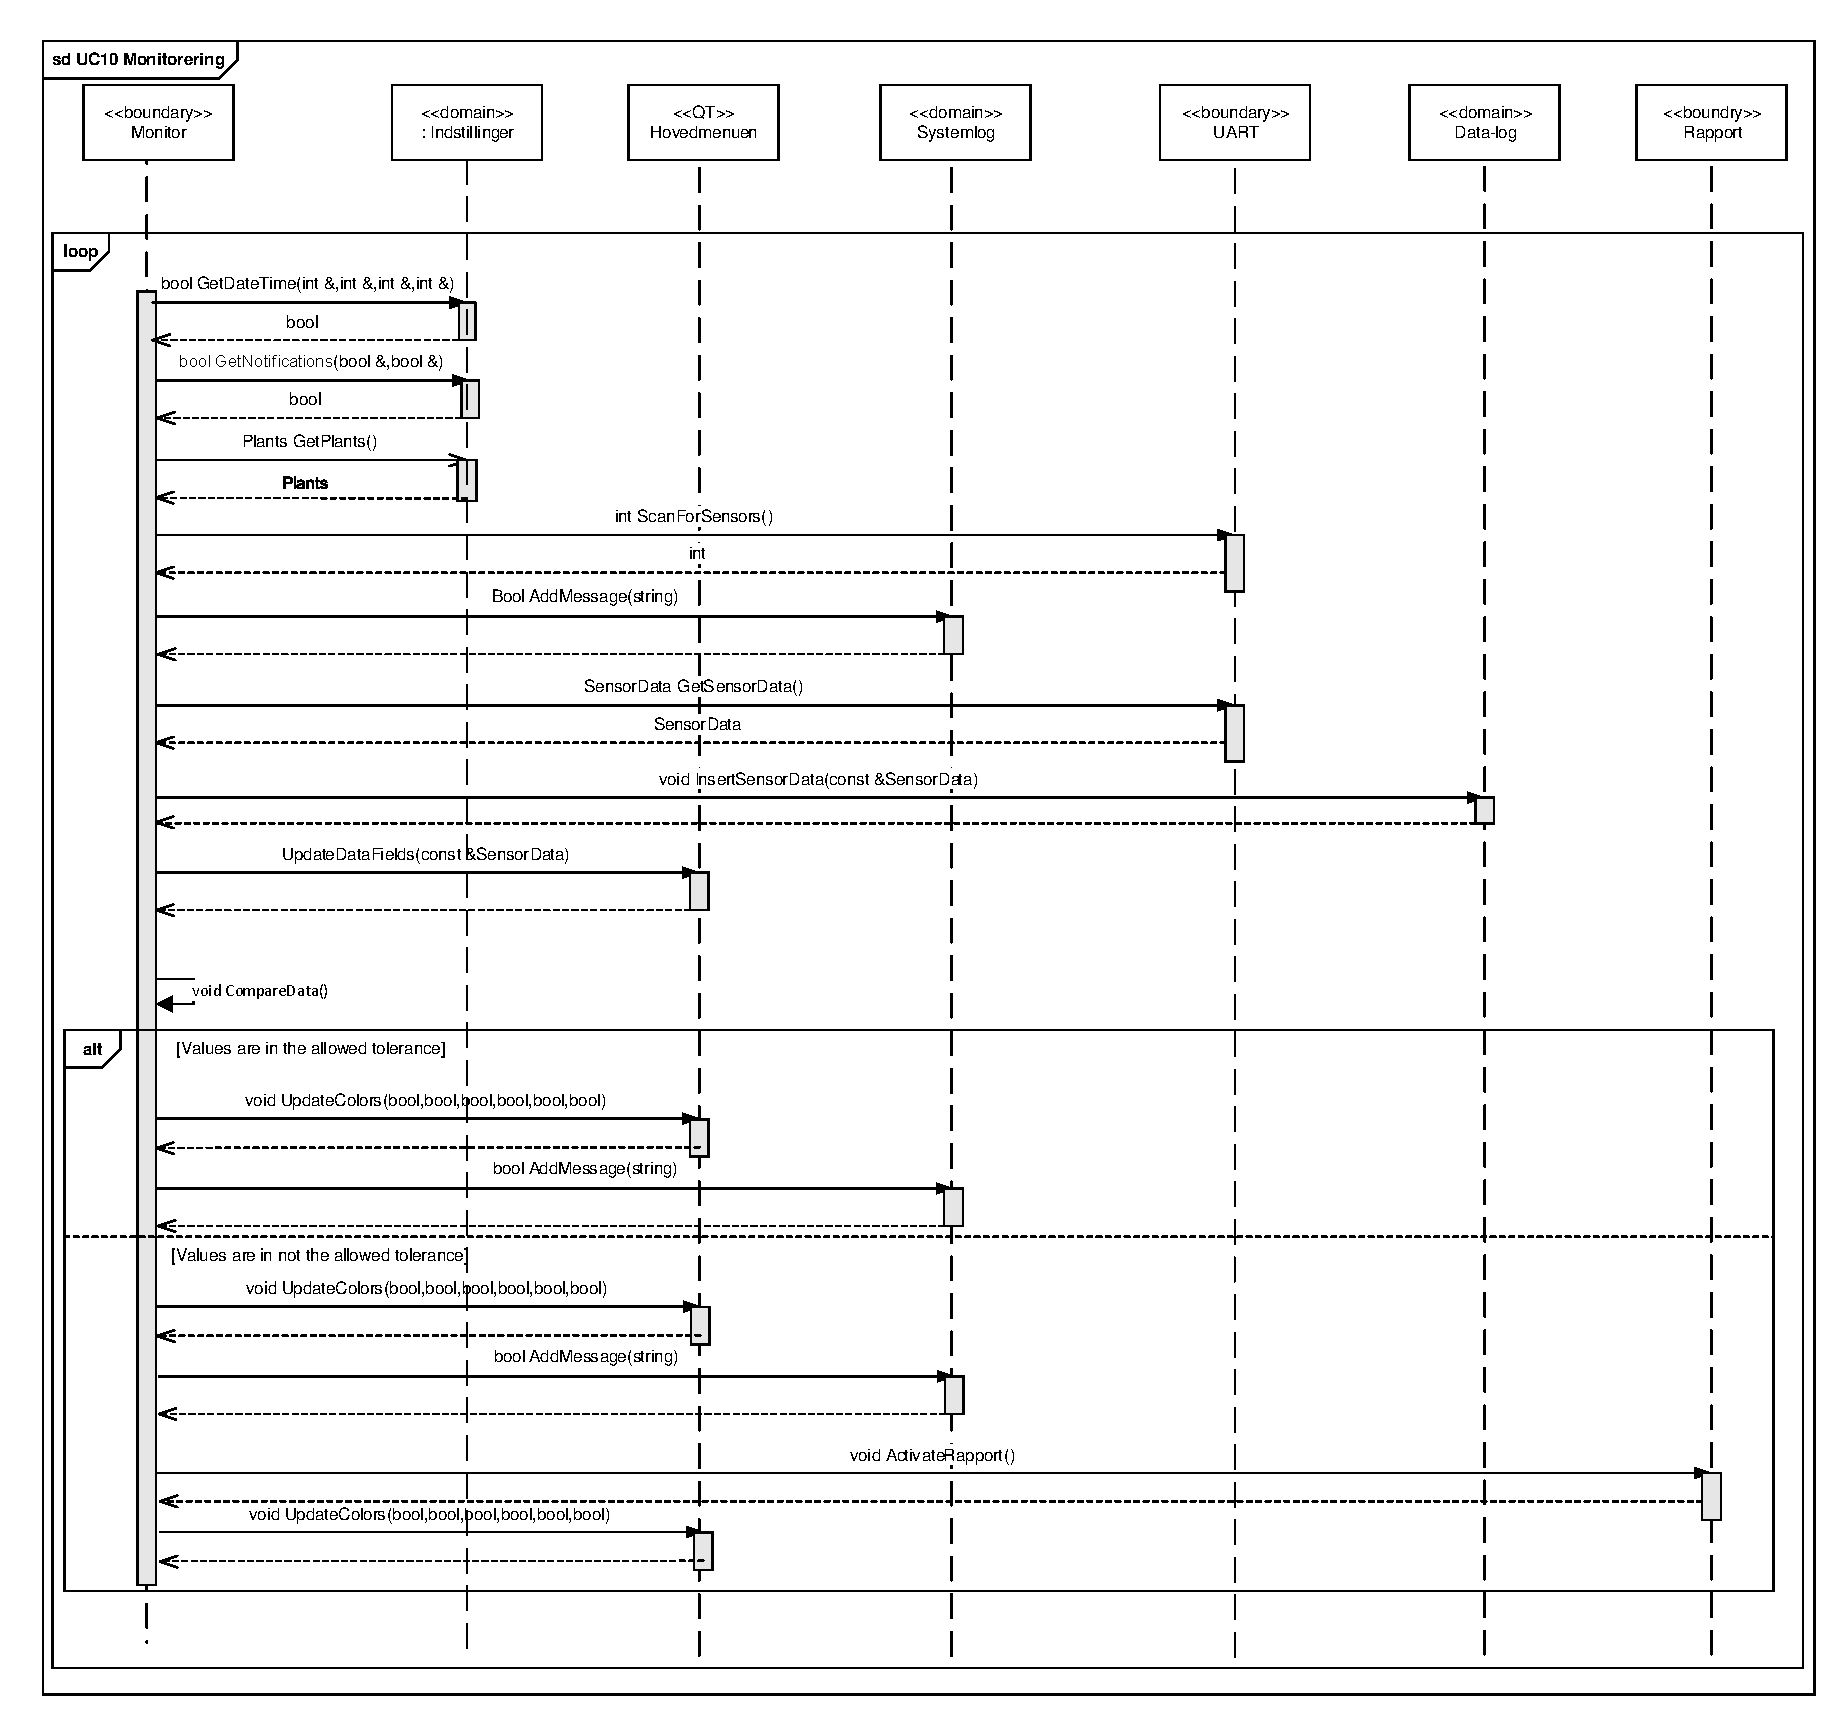
\includegraphics[width={\textwidth}, trim=0 0 0 0, clip=true] {../fig/SD_autoGreen_UC_10.pdf}
\caption{Application model for UC10: Monitorering}
\label{fig:SD_UC10}
\end{figure}

Sekvensdiagrammet giver et overblik over hvordan monitoreringstråden skal fungere, og hvilke funktionskald den skal fortage til andre klasser.

\clearpage

\subsection{Usecase 11: Regulering}

\begin{figure}[!h]
\centering 
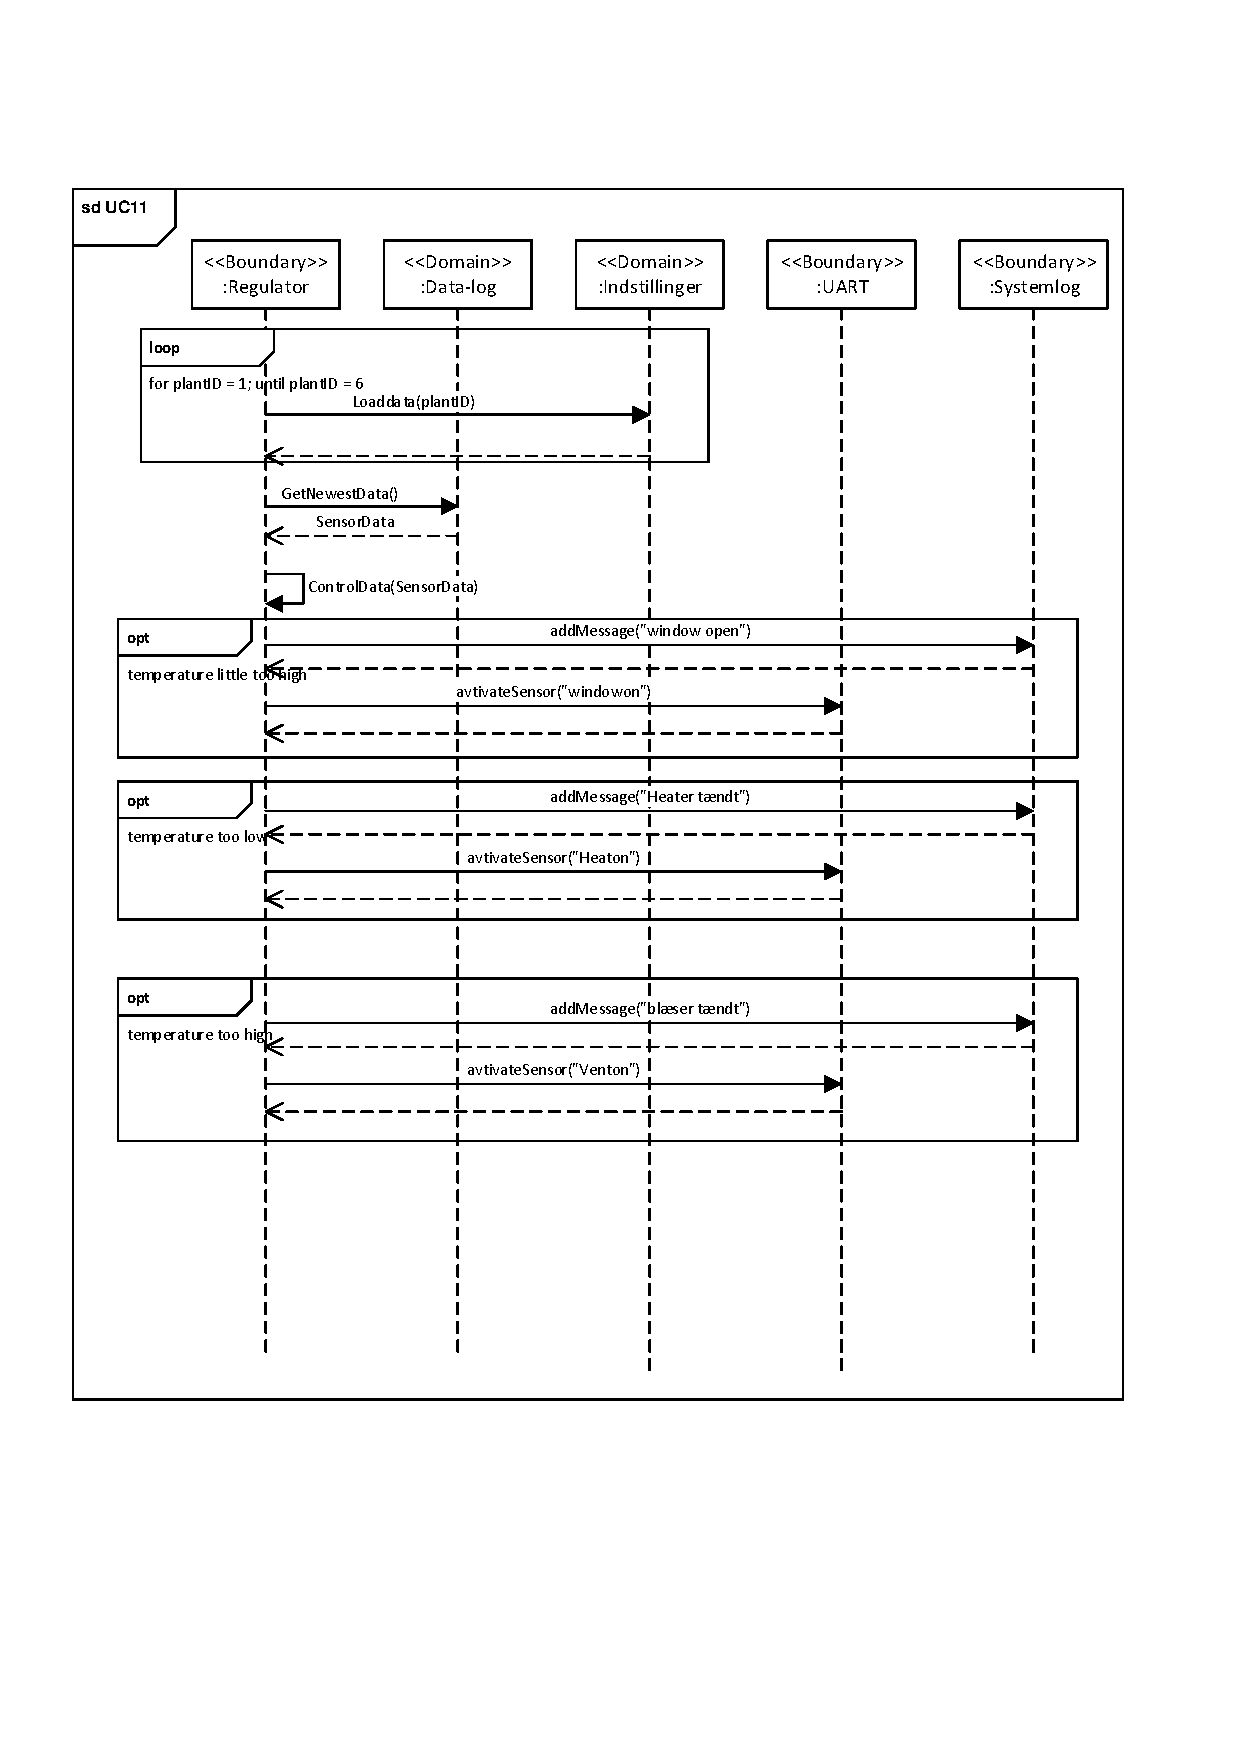
\includegraphics[width={\textwidth}, trim=0 150 0 90, clip=true]{../fig/SD_autogreen_UC_11_regulering.pdf}
\caption{Application model for UC11: Regulering}
\label{fig:SD_UC11}
\end{figure}

Sekvensdiagrammer giver overblik over hvordan reguleringstråden skal fungere, og hvilke funktionskald den skal fortage til andre klasser. f.eks. kald til UART omkring åbning eller lukning af vinduet.

\clearpage
\section{Klassebeskrivelser}

\subsection{Domainklasse Datalog}

\textbf{Attributter}

\begin{table}[h]
\begin{tabularx}{\textwidth}{| >{\raggedright\arraybackslash}X | >{\raggedright\arraybackslash}X | >{\raggedright\arraybackslash}p{10 cm} |} \hline
\texttt{DatalogList} & \texttt{datalog} & datalogList er en nedarvning af doublylinkedlist, med extra variabler til lagring af tid, temperatur, lysintensitet, luftfugtighed, og 6 jordfugtigheder. \\\hline
\end{tabularx}
\caption{Attributter for klassen Datalog}
\label{table:Datalog_attributter}
\end{table}

\textbf{Metoder}

\begin{table}[h]
\begin{tabularx}{\textwidth}{| >{\raggedright\arraybackslash}p{2.5 cm} | >{\raggedright\arraybackslash}X |} \hline
Prototype & \texttt{void GetData(int time, int temp, int light, int humidity, int ground)} \\\hline
Parametre & \texttt{int time} \newline 
time er en reference til et array som indeholder tidsstempler over en hvis periode. \newline
\texttt{int temp} \newline
temp er en reference til et array som indeholder temperaturen på de angivne tidstempler. \newline
\texttt{int light} \newline
light er en reference til et array som indeholder lysintensiteten på de angivne tidstempler. \newline
\texttt{int humidity} \newline
ground er en reference til et 2D array, hvor hver kolonne indeholde jordfugtigheden for den givne plante. Hver række indeholder jordfugtigheden på de angive tidstempler. \newline
\texttt{int ground} \newline
temp er en reference til et array som indeholder temperaturen på de angivne tidstempler. \\\hline
Returværdi & - \\\hline
Beskrivelse & Metoden har til fordel at hente data ud i et angivet tidsområde, ved at indsætte disse data ind i referencerne, hvorefter metoden afsluttes. \\\hline
\end{tabularx}
\caption{GetData}
\label{table:GetData}
\end{table}

\begin{table}[h]
\begin{tabularx}{\textwidth}{| >{\raggedright\arraybackslash}p{2.5 cm} | >{\raggedright\arraybackslash}X |} \hline
Prototype & \texttt{void InsertSensorData(const SensorData SensorData)} \\\hline
Parametre & \texttt{int time} \newline 
time er en reference til et array som indeholder tidsstempler over en hvis periode. \\\hline
Returværdi & - \\\hline
Beskrivelse & Når metoden kaldes oprettes en ny Node i den linked list hvor alt dataen fra parameteren SensorData bliver lagret i. \\\hline
\end{tabularx}
\caption{InsertSensorData}
\label{table:InsertSensorData}
\end{table}

\begin{table}[h]
\begin{tabularx}{\textwidth}{| >{\raggedright\arraybackslash}p{2.5 cm} | >{\raggedright\arraybackslash}X |} \hline
Prototype & \texttt{void GetNewestData(int temp, int humidity, int plant)} \\\hline
Parametre & \texttt{int temp} \newline 
temp er en reference til en int, som indeholder den temperatur fra den nyeste node i linked listen. \newline
\texttt{int humidity} \newline
humidity er en reference til en int, som indeholder luftfugtigheden fra den nyeste node i linked listen. \newline
\texttt{int plant} \newline
ground er en reference til et int array, som indeholde jordfugtigheden for planterne fra den nyeste node i linked listen \\\hline
Returværdi & - \\\hline
Beskrivelse & Metoden går ind i link listen fra nyeste data og går tilbage indtil at tiden passer med 24 timer før den nuværende tid, herefter tages data, 24 timer længere tilbage, og regnes sammen til en gennemsnitlig temperatur, luftfugtighed, lysintensitet og for op til 6 jordfugtigheder. De data der udtages af link listen slettes, og en ny Node oprettes på den først udtages plads. \\\hline
\end{tabularx}
\caption{GetNewestData}
\label{table:GetNewestData}
\end{table}


\begin{table}[h]
\begin{tabularx}{\textwidth}{| >{\raggedright\arraybackslash}p{2.5 cm} | >{\raggedright\arraybackslash}X |} \hline
Prototype & \texttt{void Sortweek()} \\\hline
Parametre & - \\\hline
Returværdi & - \\\hline
Beskrivelse & Metoden går ind i link listen fra nyeste data og går tilbage indtil at tiden passer med 2 dage før den nuværende tid, herefter tages data, 7 dage længere tilbage, og regnes sammen til en gennemsnitlig temperatur, luftfugtighed, lysintensitet og for op til 6 jordfugtigheder. De data der udtages af link listen slettes, og en ny Node oprettes på den først udtages plads. \\\hline
\end{tabularx}
\caption{Sortweek}
\label{table:Sortweek}
\end{table}

\begin{table}[h]
\begin{tabularx}{\textwidth}{| >{\raggedright\arraybackslash}p{2.5 cm} | >{\raggedright\arraybackslash}X |} \hline
Prototype & \texttt{void Sortmonth()} \\\hline
Parametre & - \\\hline
Returværdi & - \\\hline
Beskrivelse & Metoden går ind i link listen fra nyeste data og går tilbage indtil at tiden passer med 8 dage før den nuværende tid, herefter tages data, 30 dage længere tilbage, og regnes sammen til en gennemsnitlig temperatur, luftfugtighed, lysintensitet og for op til 6 jordfugtigheder. De data der udtages af link listen slettes, og en ny Node oprettes på den først udtages plads. \\\hline
\end{tabularx}
\caption{Sortmonth}
\label{table:Sortmonth}
\end{table}


\clearpage


%TODO Læg dette ind i samme dok?
\section{Indstillinger} \label{sec:Indstillinger_impl}

Indstillinger er en klasse, som holder styr på systemets indstillinger. Klassen kan også blive refereret til, som konfigurationsfil, enkelte steder. Klassens primære opgave er, at holde styr på tiden i systemet, de virtuelle planter i drivhuset samt hvilken hardware der må bruges til at regulere med.
Tiden kunne implementeres på et par måder. Der kunne fx laves en counter, hvor der tælles op hvert sekund. Denne løsning blev dog ikke valgt, da vi anvender en embedded linux platform, som selv kan holde styr på tiden, hvis den indstilles korrekt. Der er dog nogle krav til at indstille tiden på den embeddede linux platform. Når tiden skal indstilles, skal der bruges ”super brugerrettigheder”, altså tiden skal sættes mens root anvendes.
I Listing \ref{lst:setDate}, ses noget af koden der indstiller tiden.

\subsection{SetDate}

Koden i Listing \ref{lst:setDate} opretter en pipe til linux’s commandline, og kører kommandoen \texttt{pwd} på linux platformen, som returnerer stien programmet køres i. Denne sti bruges til at eksekvere et script med de ønskede tidsindstillinger, således tiden sættes til det rigtige på systemet. 

\lstinputlisting[linerange=setDate0-setDate1, label=lst:setDate, caption=Implementering af setDate]{../src/AutoGreenSem3/Devkit8000/autogreenbuild3/Indstillinger.hpp}

Scriptet som koden afvikler, bruger kommandoen Date, som enten kan sætte tiden eller vise den. Kommandoen Date findes i en minimal version på DevKit8000, da linux distributionen angstrom, har brugt busybox. BusyBox kombinerer bittesmå versioner af mange almindelige UNIX utilities, i en enkelt lille eksekverbar fil. Det betyder at de ikke tager hele programmet med, kun det mest nødvendige af det.  Koden kan ses i Listing \ref{lst:setTimeBeagleBoard}.

\clearpage

\lstinputlisting[linerange=setTimeBeagleBoard0-setTimeBeagleBoard1, label=lst:setTimeBeagleBoard, caption=Implementering af setTimeBeagleBoard scriptet, language=bash]{../src/AutoGreenSem3/Devkit8000/autogreenbuild3/setTimeBeagleBoard.c}

\subsection{Exec af linux kommandoer}

I metoden exec, er det kode som får platformen til at køre kommandoer i linux’s shell. Metoden tager et char array, der indeholder den kommando der ønskes afviklet på systemet, som parameter. Popen-metoden laver en proces ved at kalde pipe i read-mode, så retursvaret fra kommandoen fås i en string. Metoden kan ses i Listing \ref{lst:exec}.

\lstinputlisting[linerange=exec0-exec1, label=lst:exec, caption=Implementering af exec]{../src/AutoGreenSem3/Devkit8000/autogreenbuild3/Indstillinger.hpp}

\subsection{GetDate}
Nu da tiden kan sættes til den tid det ønskede på platformen, er det meget nemmere at læse den ud fra systemet. Fordi vi bare kan bruge et almindeligt API kald som er bygget ind i c++. I Listing \ref{lst:getDate} vises den kode, der henter tiden ud.

\lstinputlisting[linerange=getDate0-getDate1, label=lst:getDate, caption=Implementering af getDate.]{../src/AutoGreenSem3/Devkit8000/autogreenbuild3/Indstillinger.hpp}

I projektet er det valgt at repræsentere tid med en struct, der indeholder år, måneder, dage, timer og minutter. Dog skal structen først udfyldes med tiden fra systemet, hvilket gøres ved at oprette et objekt af typen time\_t med navnet ”tm”. Objektet fyldes så med systemets tid med funktionen time$(0)$. Efter dette fylder metoden tids-structen ud og returnerer denne.

\subsection{Get- og set-metoder}

Ud over disse metoder indeholder indstillinger en masse get- og set-metoder, så de andre klasser kan hente information om drivhuset. Eksempler kan ses i Listing \ref{lst:getHardware} og \ref{lst:setHardware}.

Her tages en reference til 
\lstinputlisting[linerange=GetHardware0-GetHardware1, label=lst:getHardware, caption=Implementering af getHardware.]{../src/AutoGreenSem3/Devkit8000/autogreenbuild3/Indstillinger.hpp}

\lstinputlisting[linerange=SetHardware0-SetHardware1, label=lst:setHardware, caption=Implementering af setHardware.]{../src/AutoGreenSem3/Devkit8000/autogreenbuild3/Indstillinger.hpp}

\clearpage

\subsection{Boundaryklasse Monitor}

\textbf{Attributter}

\begin{table}[h]
\begin{tabularx}{\textwidth}{| >{\raggedright\arraybackslash}X | >{\raggedright\arraybackslash}X | >{\raggedright\arraybackslash}p{10 cm} |} \hline
\texttt{CurrentTime} & \texttt{Date} & Indeholder sidste tidpunkt modtaget fra Indstillinger. \\\hline
\texttt{Email} & \texttt{Notification} & Indeholder status for rapportering. \\\hline
\texttt{Virtuel} & \texttt{Plant} & Indeholder array af virtuelle planteparametre. \\\hline
\texttt{Real} & \texttt{Plant} & Indeholder array af faktiske planteparametre. \\\hline
\end{tabularx}
\caption{Attributter for klassen Monitor}
\label{table:Monitor_attributter}
\end{table}

\textbf{Metoder}

\begin{table}[h]
\begin{tabularx}{\textwidth}{| >{\raggedright\arraybackslash}p{2.5 cm} | >{\raggedright\arraybackslash}X |} \hline
Prototype & \texttt{void CompareData()} \\\hline
Parametre & - \\\hline
Returværdi & - \\\hline
Beskrivelse & CompareDatas opgave er en live opdatering af plante sundhedstegn på baggrund af en sammenligningen mellem hvad brugeren har angivet som de ideelle værdier i den virtuelle plantedatabase og de faktiske værdier indsamlet fra sensorer. Hvis de faktiske værdier ligger inden for tolerancen vil Monitor farve plantefelterne i hovedmenuen grønne og hvis de ligger udenfor skal plantefelterne være røde. I tilfælde af en sensor ikke er tilkoblet, så skal plantefeltet for den pågældende sensor være grå.Hver gang en tolerance overskides skal Monitor angive hændelsen til systemloggen og signaler rapportering for aktivering. \\\hline
\end{tabularx}
\caption{CompareData}
\label{table:CompareData}
\end{table}

\clearpage

\subsection{Domainklasse Plantedatabase}

\textbf{Attributter}

\begin{table}[h]
\begin{tabularx}{\textwidth}{| >{\raggedright\arraybackslash}X | >{\raggedright\arraybackslash}X | >{\raggedright\arraybackslash}p{10 cm} |} \hline
\texttt{dataBase} & \texttt{DoublyLinkedList} & Datastrukturen som indeholder alle planterne \\\hline
\end{tabularx}
\caption{Attributter for klassen Plantedatabase}
\label{table:Plantedatabase_attributter}
\end{table}

\textbf{Metoder}

\begin{table}[h]
\begin{tabularx}{\textwidth}{| >{\raggedright\arraybackslash}p{2.5 cm} | >{\raggedright\arraybackslash}X |} \hline
Prototype & \texttt{Plant GetPlantList()} \\\hline
Parametre & - \\\hline
Returværdi & \texttt{Plant} \newline
Et Plant array med alle planter I database. \\\hline
Beskrivelse & Bruges til at hente all planter i databasen. \\\hline
\end{tabularx}
\caption{GetPlantList}
\label{table:GetPlantList}
\end{table}

\begin{table}[h]
\begin{tabularx}{\textwidth}{| >{\raggedright\arraybackslash}p{2.5 cm} | >{\raggedright\arraybackslash}X |} \hline
Prototype & \texttt{Plant GetPlant(int id)} \\\hline
Parametre & \texttt{int id} \newline
id nummeret for den ønskede plante. \\\hline
Returværdi & \texttt{Plant} \newline
En plante som har det givne id. \\\hline
Beskrivelse & Henter en plant ud af databasen som har det angivne id. \\\hline
\end{tabularx}
\caption{GetPlant}
\label{table:GetPlant}
\end{table}

\begin{table}[h]
\begin{tabularx}{\textwidth}{| >{\raggedright\arraybackslash}p{2.5 cm} | >{\raggedright\arraybackslash}X |} \hline
Prototype & \texttt{void InsertPlant(Plant plant)} \\\hline
Parametre & \texttt{Plant plant} \newline
Den plante som skal indsættes. \\\hline
Returværdi & - \\\hline
Beskrivelse & Indsætter en plante i databasen. \\\hline
\end{tabularx}
\caption{InsertPlant}
\label{table:InsertPlant}
\end{table}

\begin{table}[h]
\begin{tabularx}{\textwidth}{| >{\raggedright\arraybackslash}p{2.5 cm} | >{\raggedright\arraybackslash}X |} \hline
Prototype & \texttt{void DeletePlant(int id)} \\\hline
Parametre & \texttt{int id} \newline
id på planeten som skal slettes \\\hline
Returværdi & - \\\hline
Beskrivelse & Sletter en planet som har det angivende id. \\\hline
\end{tabularx}
\caption{DeletePlant}
\label{table:DeletePlant}
\end{table}

\begin{table}[h]
\begin{tabularx}{\textwidth}{| >{\raggedright\arraybackslash}p{2.5 cm} | >{\raggedright\arraybackslash}X |} \hline
Prototype & \texttt{plant CreatePlant()} \\\hline
Parametre & - \\\hline
Returværdi & \texttt{Plant} \newline
En ny plante. \\\hline
Beskrivelse & Opretter en ny plante i Datastrukturen og returnere denne plante, så det er muligt at redigere i data på den ved brug af plantedataredigeringsmenuen. \\\hline
\end{tabularx}
\caption{CreatePlant}
\label{table:CreatePlant}
\end{table}

\clearpage

\subsection{Boundaryklasse Rapport}

\textbf{Attributter}

\begin{table}[h]
\begin{tabularx}{\textwidth}{| >{\raggedright\arraybackslash}X | >{\raggedright\arraybackslash}X | >{\raggedright\arraybackslash}p{10 cm} |} \hline
\texttt{CurrentTime} & \texttt{Date} & Indeholder sidste tidpunkt modtaget fra Indstillinger. \\\hline
\texttt{Email} & \texttt{Notification} & Indeholder maillingsliste for status emails \\\hline
\end{tabularx}
\caption{Attributter for klassen Rapport}
\label{table:Rapport_attributter}
\end{table}

\textbf{Metoder}

\begin{table}[h]
\begin{tabularx}{\textwidth}{| >{\raggedright\arraybackslash}p{2.5 cm} | >{\raggedright\arraybackslash}X |} \hline
Prototype & \texttt{void ActivateRapport()} \\\hline
Parametre & - \\\hline
Returværdi & - \\\hline
Beskrivelse & Sendes fra Monitor og angiver om rapporterings funktionaliteter skal bruges eller ej. \\\hline
\end{tabularx}
\caption{ActivateRapport}
\label{table:ActivateRapport}
\end{table}

\begin{table}[h]
\begin{tabularx}{\textwidth}{| >{\raggedright\arraybackslash}p{2.5 cm} | >{\raggedright\arraybackslash}X |} \hline
Prototype & \texttt{void SendDailyRapport()} \\\hline
Parametre & - \\\hline
Returværdi & - \\\hline
Beskrivelse & Sender en E-mail til brugeren med en liste over de seneste systemhændelser siden sidste E-mail. \\\hline
\end{tabularx}
\caption{SendDailyRapport}
\label{table:SendDailyRapport}
\end{table}

\begin{table}[h]
\begin{tabularx}{\textwidth}{| >{\raggedright\arraybackslash}p{2.5 cm} | >{\raggedright\arraybackslash}X |} \hline
Prototype & \texttt{void SendWarningRapport()} \\\hline
Parametre & - \\\hline
Returværdi & - \\\hline
Beskrivelse &  Sender en E-mail til brugeren med den kritiske systemhændelse. \\\hline
\end{tabularx}
\caption{SendWarningRapport}
\label{table:SendWarningRapport}
\end{table}

\clearpage

\subsection{Boundaryklasse Regulator}

\textbf{Attributter}

\begin{table}[h]
\begin{tabularx}{\textwidth}{| >{\raggedright\arraybackslash}X | >{\raggedright\arraybackslash}X | >{\raggedright\arraybackslash}p{10 cm} |} \hline
\texttt{TempHigh} & \texttt{bool} & som standard står TempHigh som False, men hvis temperature bliver for høj sættes den True. \\\hline
\texttt{TempLow} & \texttt{bool} & som standard står TempLow som False, men hvis temperature bliver for lav sættes den True. \\\hline
\texttt{humidityLow} & \texttt{bool} & som standard står humidityLow som False, men hvis luftfugtigheden bliver for lav sættes den True. \\\hline
\texttt{humidityHigh} & \texttt{bool} & som standard står humidityHigh som False, men hvis luftfugtigheden bliver for høj sættes den True.\\\hline
\texttt{plante1water 1-6} & \texttt{bool} & Plante(1-6)water står som standard til False, men hvis jordfugtigheden bliver 2 niveauer for lavt sættes den til True.\\\hline
\end{tabularx}
\caption{Attributter for klassen Regulator}
\label{table:Regulator_attributter}
\end{table}

\textbf{Metoder}

\begin{table}[h]
\begin{tabularx}{\textwidth}{| >{\raggedright\arraybackslash}p{2.5 cm} | >{\raggedright\arraybackslash}X |} \hline
Prototype & \texttt{void ControlData()} \\\hline
Parametre & - \\\hline
Returværdi & - \\\hline
Beskrivelse & Metoden har til formål at sammenligne den faktiske temperatur i drivhuset med den ønskede temperatur. Det samme fortages med luftfugtighed. I forhold til jordfugtigheden tjekkes hver plante, og hvis jordfugtigheden er for lav, sættes boolean til at den gældende plante mangler vand. \\\hline
\end{tabularx}
\caption{ControlData}
\label{table:ControlData}
\end{table}

\clearpage

\subsection{Domainklasse Systemlog}

\textbf{Attributter}

\begin{table}[h]
\begin{tabularx}{\textwidth}{| >{\raggedright\arraybackslash}X | >{\raggedright\arraybackslash}X | >{\raggedright\arraybackslash}p{10 cm} |} \hline
\texttt{SystemMsg} & \texttt{DoublyLinkedList} & SystemMsg implementeres som en struct, der nedarver fra Node klassen, og udvider dem med en message item af typen string. \\\hline
\end{tabularx}
\caption{Attributter for klassen Systemlog}
\label{table:Systemlog_attributter}
\end{table}

\textbf{Metoder}

\begin{table}[h]
\begin{tabularx}{\textwidth}{| >{\raggedright\arraybackslash}p{2.5 cm} | >{\raggedright\arraybackslash}X |} \hline
Prototype & \texttt{void AddMessage(string msg)} \\\hline
Parametre & \texttt{string msg} \newline
string msg er en besked indeholdende den pågældende systemhændelse formateret på følgende måde: ”klassenavn”: ”hændelse” på ”tidspunkt”. \\\hline
Returværdi & - \\\hline
Beskrivelse & Funktionen har til formål at modtage systembeskeder fra andre klasser og indsætte disse beskeder i en datastruktur til senere brug. \\\hline
\end{tabularx}
\caption{AddMessage}
\label{table:AddMessage}
\end{table}

\begin{table}[h]
\begin{tabularx}{\textwidth}{| >{\raggedright\arraybackslash}p{2.5 cm} | >{\raggedright\arraybackslash}X |} \hline
Prototype & \texttt{void PrintSystemLog()} \\\hline
Parametre & - \\\hline
Returværdi & - \\\hline
Beskrivelse & PrintSystemLog bliver kaldt fra QT menuen ”Systemlogmenu” og udskriver de sidste 5 systemhændelser med den femte ældste hændelse først og den nyeste hændelse sidst. \\\hline
\end{tabularx}
\caption{PrintSystemLog}
\label{table:PrintSystemLog}
\end{table}

\clearpage

\subsection{Boundaryklasse UART}

\textbf{Attributter} %TODO

\begin{table}[h]
\begin{tabularx}{\textwidth}{| >{\raggedright\arraybackslash}X | >{\raggedright\arraybackslash}X | >{\raggedright\arraybackslash}p{10 cm} |} \hline
\texttt{SystemMsg} & \texttt{DoublyLinkedList} & SystemMsg implementeres som en struct, der nedarver fra Node klassen, og udvider dem med en message item af typen string. \\\hline
\end{tabularx}
\caption{Attributter for klassen UART}
\label{table:UART_attributter}
\end{table}

\textbf{Metoder}

\begin{table}[h]
\begin{tabularx}{\textwidth}{| >{\raggedright\arraybackslash}p{2.5 cm} | >{\raggedright\arraybackslash}X |} \hline
Prototype & \texttt{void ScanForSensors()} \\\hline
Parametre & - \\\hline
Returværdi & - \\\hline
Beskrivelse & metoden sender en besked til PSoC masteren og beder om antallet af tilsluttede sensorer til systemet. UARTen sender kommandoen (REF til UART protokol), og venter derefter på svar fra PSoC masteren. Hvis den får et gyldigt svar tilbage afsluttes metoden. Hvis svaret ikke er gyldigt vil metoden kontakte PSoC masteren en gang til for at få antallet af tilsluttede sensorer. Efter 4 fejlforsøg afsluttes metoden, og systemet sender en besked til bruger at tjekke systemet. \\\hline
\end{tabularx}
\caption{ScanForSensors}
\label{table:ScanForSensors}
\end{table}

\begin{table}[h]
\begin{tabularx}{\textwidth}{| >{\raggedright\arraybackslash}p{2.5 cm} | >{\raggedright\arraybackslash}X |} \hline
Prototype & \texttt{SensorData GetSensorData() } \\\hline
Parametre & - \\\hline
Returværdi &\texttt{SensorData} \newline
SensorData, som er en struct over temperatur, luftfugtighed, lysintensitet og jordfugtighed returneres med værdierne for målt temperatur, luftfugtighed, lysintensitet og jordfugtighed. \\\hline
Beskrivelse & metoden sender via UART protokollen en anmodning til PSoC masteren om at få temperaturen i drivhuset. Når korrekt data er modtaget fortsætter metoden til at indsamle data for luftfugtighed, lysintensitet og jordfugtighed for de 6 planter. Hvis en fejl i en af beskederne opstår, forsøges yderlige 3 forsøg for den gældte data, før den springer den gældende data over og fortsætter til næste data.  \\\hline
\end{tabularx}
\caption{GetSensorData}
\label{table:GetSensorData}
\end{table}

\clearpage

\subsection{Threads}
For at kunne afvikle flere funktionaliteter på samme tid i systemet bruges multithreading. Ved at bruge en thread til brugerfladen, en til at læse data, en til at regulere klimaet, hvis data ligger er for langt uden for tolerancer niveauer og en til at styrer tiden med, kan de forskellige funktionaliteter kører sideløbende.












